\documentclass[a4paper,12pt]{article}

\usepackage{cmap}
\usepackage{mathtext}
\usepackage[T2A]{fontenc}
\usepackage[utf8]{inputenc}
\usepackage[english,russian]{babel}

\usepackage{amsmath,amsfonts,amssymb,amsthm,mathtools}
\usepackage{icomma}
\usepackage{upgreek}
\mathtoolsset{showonlyrefs=true}

\usepackage{tabto}
\usepackage{euscript}
\usepackage{mathrsfs}

\usepackage{graphicx}

\newcommand*{\hm}[1]{#1\nobreak\discretionary{}
{\hbox{$\mathsurround=0pt #1$}}{}}

\author{Kupriyanov Kirill}
\title{Data Analysis PI\\Theoretical assignment $\#3$}
\date{}

\begin{document}
\maketitle
\thispagestyle{empty}
\newpage
\section*{Task 1.}
\underline{\textit{Problem:}} Consider linear regression task in
one-dimensional space. \({(x_i , y_i)}^N_{i=1}\) is a training dataset and
for object \(i: x_i \in [-1, 1]\) is a feature, $y_i$ is an answer we want to
predict, $y_i^*=kx_i+b$ is our prediction. At the picture below you can see
three different plots of the prediction error \((y - y^*)\) against $x$. Which of
these plots cannot be obtained if least squares method is used to train a
regression model?\\
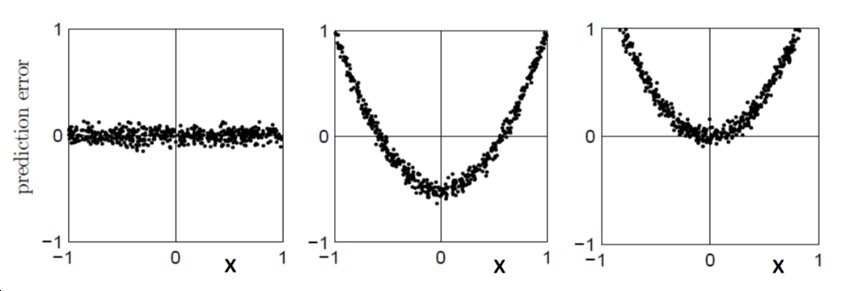
\includegraphics[width=\textwidth]{1}
\newline
\underline{\textit{Solution:}} The first picture represents how data is spread very linearly, obviously, this situation can exist.\\
Pictures 2 and 3 are representing non-linear, but but kind of uniformly
distributed dependencies of features. Also these distributions could roughly be described with the following equation: \(y - \hat{y} = x^2+b\)
\begin{gather}
    y - \hat{y} = x^2 + b\\
    (y - \hat{y})^2 = (x^2 + b^2)^2\\
    \text{OLS: } \sum^{N}_{i = 1}{(y_i - \hat{y_i})^2} \rightarrow \text{min}\\
    \int_{-1}^{1} (y - \hat{y})^2  \rightarrow \text{min}\\
    F((x^2+b)^2) = \frac{x^5}{5} + 2b\frac{x^3}{3} + xb^2\\
    \int_{-1}^{1}(x^2 + b)^2 = \frac{1}{5}+\frac{2b}{3} + b^2 + \frac{1}{5} + \frac{2}{3}b + b^2 = \frac{2}{5} + \frac{4}{3}b + 2b^2
\end{gather}
Taking derivative, there comes a value of $b$, with which integral reaches tis minimum ponts.
\begin{gather}
    4b + \frac{4}{3} = 0\\
    b = -\frac{1}{3}
\end{gather}\\
So we get  $x^2 - \frac{1}{2}$. Second picture is more likely to be chosen than the trird one. 


The construction time of a balanced
decision tree is \(O(N\cdot D\cdot \log(N))\). The algorithm attempts to build
the balanced tree, but often does not succeed, nevertheless, assuming that
subtrees are approximately balanced, the cost at each node consists of
searching through all (\(O(D)\)) features to find one that offers the largest
reduction in the entropy. That thing has computational complexity of
\(O(N\cdot D \cdot \log(N))\). If operations at each node are summed up, the
result is \(O(N^2\cdot D\cdot \log(N))\). \\
\newline
\textit{And I think that there is a mistake in the problem statement: it was meant to be written \(O(N^2\cdot D\cdot \log(N))\)} but instead it says $D^2$..

\newpage
\section*{Task 2.}
\underline{\textit{Problem:}} Assume we use a particular feature \(i\) for
splitting a certain internal node containing \(N\) objects. We
want to determine the optimal threshold value \(h
\) such that the sum of entropies for the children nodes
\(\{x|x\cdot i < h\} \text{ and } \{x|x\cdot i > h\}\) is the smallest. Propose the algorithm that founds the optimal threshold
with complexity \(O(N\cdot \log(N))\).\\
\newline
\underline{\textit{Solution:}} Implementation from the previous task does
overhead. It recomputes class labels at each new split. What could be done is
presorting features over all relevant samples while keeping the label count. It
will reduce the complexity at each node to \(O(N\cdot \log(N))\). Finding
optimal sum of entropies for 2 new child nodes takes \(O(N)\). Entropy for one
node can be calculated within \(O(1)\).\\
So the total cost for all features is \(O(N\cdot D\cdot \log(N))\). And it finds optimal threshold within \(O(N\cdot \log(N))\).

\section*{Task 3.}
\underline{\textit{Problem:}} Consider multiclass
classification task with \(K\) classes. Objects in this task have \(L\) binary
features.  How many different decision trees of depth \(L\) can be constructed
for this task? Two decision trees are different if there is an object in \(\{0,
1\}\) \(L\) which they classify differently.\\
\newline
\underline{\textit{Solution:}} If only binary features are considered and a
binary classification task, then for a training dataset having $L$ features
there are at most \(2^L\) possible instances. Taking into account that there
are $K$ classes in the dataset, there are \(2^{K^L}\) different ways of labeling
all instances, and each labeling corresponds to a different underlying boolean
function that can be represented as a decision tree.

\end{document}

% EOF
